% !TEX root = ../BeamerTemplate.tex
%%%%%%%%%%%%%%%%%%%%%%%%%%%%%%%%%%%%%%%%%%%%%%%%%%%%%%%%%%%%%%%%%%%%%%%%%%%%%%%%%%

\section{Methodology and Model Validation}

\subsection{Design and Physical Characterization}

\begin{frame}[t]{Methodology: One Physical Question, Three Numerical Views}
\centering
\begin{tikzpicture}[node distance=0.50cm and 0.58cm,>=latex,font=\scriptsize]
  \node[draw=Blue,fill=SoftBlue,rounded corners,minimum width=2.55cm,
        minimum height=0.85cm,align=center] (design) {patch feed +\\$20\!\times\!20$ lens};
  \node[draw=Teal,fill=SoftTeal,rounded corners,minimum width=2.55cm,
        minimum height=0.85cm,align=center,right=of design] (geom) {$3\!\times\!3$ angular geometry\\with / without lens};

  \node[draw=Blue,rounded corners,fill=white,minimum width=2.50cm,
        minimum height=0.78cm,align=center,below left=0.75cm and 1.05cm of geom] (sbr) {HFSS SBR+\\ray tracing + PO};
  \node[draw=Teal,rounded corners,fill=white,minimum width=2.50cm,
        minimum height=0.78cm,align=center,below=0.75cm of geom] (hybrid) {HFSS Hybrid\\FEM + SBR+};
  \node[draw=Gold!85!black,rounded corners,fill=white,minimum width=2.50cm,
        minimum height=0.78cm,align=center,below right=0.75cm and 1.05cm of geom] (sionna) {Sionna-RT\\path-based RT};

  \node[draw=Blue,fill=SoftBlue,rounded corners,minimum width=2.75cm,
        minimum height=0.85cm,align=center,below=1.05cm of hybrid] (csi) {common-format $\mathbf H(f)$\\37 / 38 / 39~GHz};
  \node[draw=Teal,fill=SoftTeal,rounded corners,minimum width=3.10cm,
        minimum height=0.85cm,align=center,right=0.65cm of csi] (metrics) {gain + correlation + SVD\\conditioning + rank + capacity};

  \draw[->,thick] (design)--(geom);
  \draw[->,thick] (geom)--(sbr);
  \draw[->,thick] (geom)--(hybrid);
  \draw[->,thick] (geom)--(sionna);
  \draw[->,thick] (sbr)--(csi);
  \draw[->,thick] (hybrid)--(csi);
  \draw[->,thick] (sionna)--(csi);
  \draw[->,thick] (csi)--(metrics);
\end{tikzpicture}

\vspace{0.45cm}
\begin{columns}[T,onlytextwidth]
  \column{0.48\textwidth}
  \MethodNote{\textbf{Controlled comparison:} identical channel convention,
  anchor frequencies, and lens/no-lens pairing.}
  \column{0.48\textwidth}
  \CautionNote{\textbf{Validation claim:} solver-robust trend; not numerical
  interchangeability and not experimental validation.}
\end{columns}
\SourceNote{Chapter 2: Methodology and Model Validation}
\note{
  \begin{itemize}
    \item These are Methodology flow for validation and model verification
    \item In this section we evaluate, is Antenna Lens realy work for channel decorrelation and spatial multiplexing enhancement
    \item So we begin Design Patch Feed, and antenna lens
    \item We put antenna lens in 3x3 angular geometry, and we evaluate with three different solver, HFSS SBR+, HFSS Hybrid, and Sionna-RT
    \item then we get the canonical H(f) and evaluate with different metrics, gain, correlation, SVD, conditioning, rank and capacity
  \end{itemize}
}
\end{frame}


\begin{frame}[t]{Patch Feed: Linking Fields to 38~GHz Performance}
\begin{columns}[T,onlytextwidth]
  \column{0.42\textwidth}
  \begin{block}{Field-to-link relation}
    \centering\scriptsize
    $P_R\propto r^{-2}
    \left|\mathbf F_R^{\mathsf H}\mathbf F_T\right|^2$

    \tiny spreading $\times$ directional/polarization overlap
  \end{block}
  \scriptsize
  \begin{itemize}
    \setlength{\itemsep}{0.05em}
    \item \textbf{Matched at 38~GHz:} resonance near 38.1~GHz,
          $S_{11}\approx-35$~dB; approximate $-10$-dB band of
          36.9--39.5~GHz.
    \item \textbf{Directional feed:} the 3D and $\phi=90^\circ$ cuts show a
          dominant forward response with weaker back radiation.
    \item \textbf{Scope:} this patch illuminates the lens characterization;
          Chapter~3 uses ideal isotropic TX patterns for controlled trajectories.
  \end{itemize}

  \column{0.54\textwidth}
  \centering
  
\includegraphics[width=\linewidth,height=2.08cm,keepaspectratio]{AntennaAndPattern.PNG}
  \begin{columns}[T,onlytextwidth]
    \column{0.57\textwidth}
      \centering
      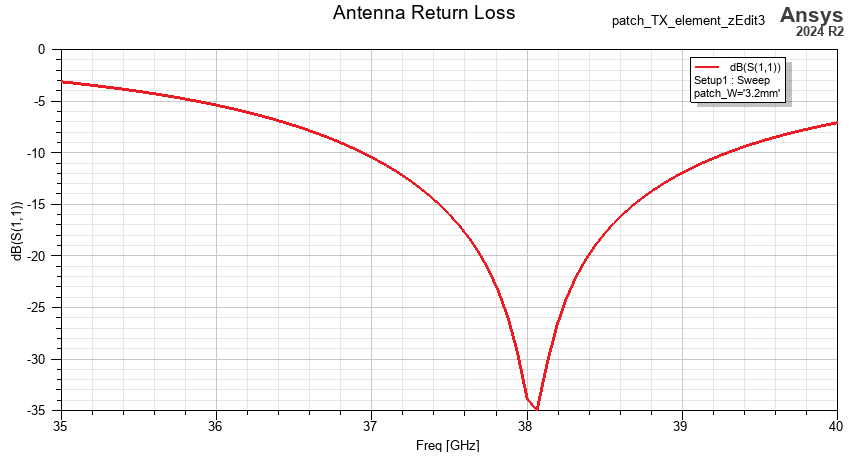
\includegraphics[width=\linewidth,height=1.80cm,keepaspectratio]{AntennaPatchReturnLoss.png}
    \column{0.41\textwidth}
      \centering
      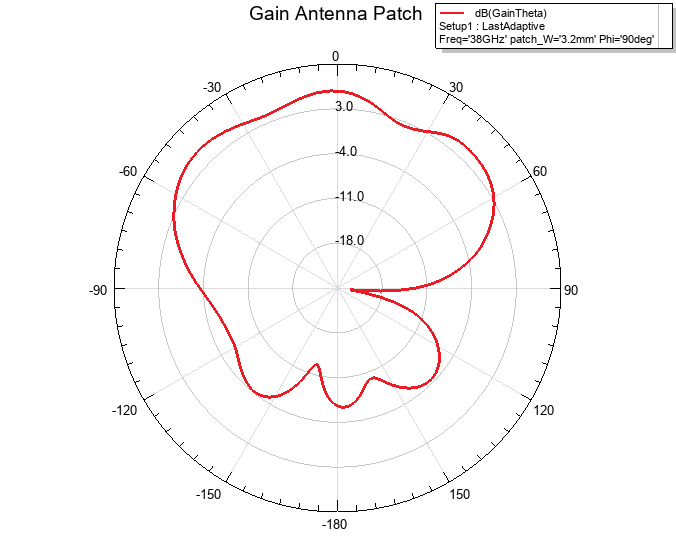
\includegraphics[width=\linewidth,height=1.80cm,keepaspectratio]{GainThetaAntennaPatch.png}
  \end{columns}
  \ThesisFigureCaption{2-1}{Patch geometry and 3D pattern, return loss, and
  $\phi=90^\circ$ gain cut at 38~GHz.}
\end{columns}
\note{
  \begin{itemize}
    \item Figure 2-1 combines the physical antenna model, its
          impedance match, and the 38~GHz angular response.
    \item The return-loss minimum occurs near 38.1~GHz at approximately
          $-35$~dB. The plotted $-10$-dB band is approximately
          36.9--39.5~GHz, so 38~GHz is well matched.
    \item The 3D and $\phi=90^\circ$ cuts show a dominant forward response with
          weaker back radiation, suitable for illuminating the transmitarray.
    \item This physical patch belongs to the lens characterization. The
          controlled Chapter~3 trajectory study intentionally uses ideal
          isotropic TX elements.
  \end{itemize}
}
\end{frame}


\begin{frame}[t]{Metasurface Unit Cell: Architecture and Floquet Setup}
\begin{columns}[T,onlytextwidth]
  \column{0.39\textwidth}
  \centering
  \begin{columns}[T,onlytextwidth]
    \column{0.34\textwidth}
      
\includegraphics[height=1.72cm]{Unitcell_Design.png}
    \column{0.63\textwidth}
      
\includegraphics[width=\linewidth,height=1.72cm,keepaspectratio]{Unitcell_Design_geometry.png}
  \end{columns}
  \ThesisFigureCaption{2-2}{Five-layer unit cell and swept geometry.}

  \vspace{0cm}
  \scriptsize\raggedright
  \begin{itemize}
    \setlength{\itemsep}{-0.12em}
    \item \textbf{Material:} Rogers RT/duroid 5880LZ,
          $\varepsilon_r=2.2$, substrate thickness $h=0.787$~mm.
    \item \textbf{Stack:} five patterned layers with
          $g_{\mathrm{air}}=1$~mm gaps.
    \item Swept $L$ and $W_{\mathrm{ind}}$ control transmission magnitude and
          phase.
  \end{itemize}

  \column{0.57\textwidth}
  \centering
  \begin{columns}[T,onlytextwidth]
    \column{0.24\textwidth}
      \centering
\includegraphics[width=\linewidth,height=2.70cm,keepaspectratio]{FloqBoundary-1.png}
      \SlideCaption{periodic 1}
    \column{0.24\textwidth}
      \centering
\includegraphics[width=\linewidth,height=2.70cm,keepaspectratio]{FloqBoundary-2.png}
      \SlideCaption{periodic 2}
    \column{0.24\textwidth}
      \centering
\includegraphics[width=\linewidth,height=2.70cm,keepaspectratio]{FloqPort-1.png}
      \SlideCaption{port 1}
    \column{0.24\textwidth}
      \centering
\includegraphics[width=\linewidth,height=2.70cm,keepaspectratio]{FloqPort-2.png}
      \SlideCaption{port 2}
  \end{columns}
  \vspace{0cm}
  \MethodNote{\textbf{Figure 2-3:} periodic boundaries + Floquet
  ports emulate plane-wave excitation and generate the transmission library.}
\end{columns}
\note{
  \begin{itemize}
    \item I implement Kanghyeok Lee's design for unitcell, his paper is Broadband metasurface superstrate for polarization-independent wave focusing and gain enhancement at Ka-band(28-32Ghz)
    \item it can using on vertical and horizontal polarization. But in this thesis, we only use vertical polarization
    \item The implemented unit cell uses Rogers RT/duroid 5880LZ with a
          substrate thickness of 0.787~mm and relative permittivity
          $\varepsilon_r=2.2$; its five patterned layers are separated by
          1~mm air gaps.
    \item This unit cell design is the most flexible unit cell design that i found so far.
    \item The adopted topology was reported as a broadband,
          polarization-independent Ka-band design \cite{Lee2022}; this thesis
          uses the vertical-polarization response.
  \end{itemize}
}
\end{frame}


\begin{frame}[t]{Transmission Library: Efficiency and Phase Coverage}
\begin{columns}[T,onlytextwidth]
  \column{0.35\textwidth}
  \tiny
  \begin{align*}
    |S_{11}|^2+|S_{21}|^2+P_{\mathrm{loss}}&=1,\\
    \eta_{\mathrm{trans}}=|S_{21}|^2&=10^{S_{21,\mathrm{dB}}/10},\\[-2pt]
    \eta_{\mathrm{refl}}=|S_{11}|^2&=10^{S_{11,\mathrm{dB}}/10}.
  \end{align*}
  \begin{block}{Selection at 38~GHz}
    \centering
    \large $S_{21}>-5\,\mathrm{dB}$\\[-1pt]
    \scriptsize $P_T>31.6\%$
  \end{block}
  \scriptsize
  \textbf{Accepted library:} 324 geometries with an approximately
  $258^\circ$ wrapped-phase span at 38~GHz. This broadens design flexibility,
  but does not provide complete $360^\circ$ coverage.

  \column{0.61\textwidth}
  \centering
  
\includegraphics[width=\linewidth,height=2.20cm,keepaspectratio]{UnitCellProfile_Magnitude_Accepted.png}
  \vspace{0.05cm}
  
\includegraphics[width=\linewidth,height=2.20cm,keepaspectratio]{UnitCellProfile_PhaseAt38GHz_Accepted.png}
  \ThesisFigureCaption{2-4}{Magnitude and wrapped phase of the 324 geometries
  accepted using $S_{21}>-5$~dB at 38~GHz.}
\end{columns}
% % \Takeaway{Use only phase states that also satisfy the transmission-efficiency
% criterion.}
\SourceNote{Chapter 2: Metasurface Unit-Cell Design}
\note{
  \begin{itemize}
    \item Figure 2-4 shows only the 324 geometries that satisfy
          $S_{21}>-5$~dB at the 38~GHz design frequency.
    \item At the threshold, the transmitted-power fraction is
          $10^{-5/10}=0.316$, so every retained state transmits more than 31.6\%.
    \item The wrapped phase extends from approximately $-58^\circ$ to
          $-316^\circ$, giving a span of about $258^\circ$.
    \item The correct claim is broader design flexibility, not complete
          $360^\circ$ phase coverage. Residual phase quantization remains.
  \end{itemize}
}
\end{frame}


\begin{frame}[t]{From Required Phase to the Realized $20\times20$ Lens}
\begin{columns}[T,onlytextwidth]
  \column{0.43\textwidth}
  \scriptsize
  \begin{equation*}
    \begin{aligned}
      d(x,y)&=\sqrt{(x-x_f)^2+(y-y_f)^2+f^2},\\
      \phi(x,y)&=\frac{2\pi}{\lambda_0}\,[d(x,y)-f]+\phi_{\mathrm{init}}.
    \end{aligned}
  \end{equation*}
  \scriptsize
  The phase mask compensates path-length differences; the finite cell library
  discretizes the continuous profile \cite{Al-Joumayly2011}.

  \vspace{0cm}
  {\scriptsize
  \renewcommand{\arraystretch}{0.76}
  \begin{tabularx}{\linewidth}{@{}Xr@{}}
    \toprule
    \textbf{Parameter} & \textbf{Value}\\
    \midrule
    Array size & $20\times20$\\
    Aperture & $44.24\times44.24$~mm$^2$\\
    Layers & 5\\
    Target focal distance & 30~mm\\
    Realized focus & $\approx14$~mm\\
    \bottomrule
  \end{tabularx}}

  \column{0.27\textwidth}
  \centering
  
\includegraphics[height=1.70cm,width=\linewidth,keepaspectratio]{AntennaLensFrontView.PNG}
  \ThesisFigureCaption{2-5}{Discrete radial state map.}
  \vspace{0.08cm}
  
\includegraphics[height=1.70cm,width=\linewidth,keepaspectratio]{AntennaLensTopView_edited.PNG}
  \ThesisFigureCaption{2-6}{Physical transmitarray layout.}

  \column{0.26\textwidth}
  \centering
  
\includegraphics[height=4.00cm,width=\linewidth,keepaspectratio]{AntennaLens20x20_VerifFocalPoint.png}
  \ThesisFigureCaption{2-7}{Axial E-field contraction.}
\end{columns}
\Takeaway{The realized focus is $\approx14$~mm versus the 30~mm target; the
thesis attributes this offset to phase quantization.}
\note{
  \begin{itemize}
    \item And after found out unit-cell profil, we design the lens with 20x20 element, and the target focal distance is 30mm, but the realized focal distance is 14mm, because of phase quantization
  \end{itemize}
}
\end{frame}


\begin{frame}[t]{Angular Focusing Traces a Focal Arc}
\centering
\begin{tabular}{@{}ccccc@{}}
  
\includegraphics[height=3.68cm]{FocalCharacter_0deg.png} &
  
\includegraphics[height=3.68cm]{FocalCharacter_m15degdeg.png} &
  
\includegraphics[height=3.68cm]{FocalCharacter_m30deg.png} &
  
\includegraphics[height=3.68cm]{FocalCharacter_m45deg.png} &
  
\includegraphics[height=3.68cm]{FocalCharacter_m60deg.png} \\
  {\scriptsize $0^\circ$} & {\scriptsize $-15^\circ$} &
  {\scriptsize $-30^\circ$} & {\scriptsize $-45^\circ$} &
  {\scriptsize $-60^\circ$}
\end{tabular}
\ThesisFigureCaption{2-8}{Focal-plane response for incidence angles from
$0^\circ$ to $-60^\circ$.}

\vspace{0.08cm}
\begin{columns}[T,onlytextwidth]
  \column{0.48\textwidth}
  \MethodNote{The energy peak shifts laterally while remaining at approximately
  the same radial distance: a \textbf{focal arc}.}
  \column{0.48\textwidth}
  \CautionNote{Focus is sharpest near $0^\circ$ and $-15^\circ$; diffuse peaks
  and sidelobes increase toward $-60^\circ$.}
\end{columns}
\SourceNote{Chapter 2: Focal Characteristics}
\note{
  \begin{itemize}
    \item This Near-field patterns Confirm the angle-dependent steering, and the energy peak shifts laterally while remaining at approximately the same radial distance: a focal arc
    \item Focus is sharpest near $0^\circ$ and $-15^\circ$; diffuse peaks and sidelobes increase toward $-60^\circ$. it also spoiled by Al-Joumayly2011 in his paper on incident at 45degree, the focus is not sharp, and the sidelobe is very high
  \end{itemize}
}
\end{frame}


\begin{frame}[t]{3D Far-Field Patterns Confirm Angle-Dependent Steering}
\centering

\includegraphics[width=0.74\linewidth,height=4.75cm,keepaspectratio]
  {AntennaPatternWithLens.png}
\ThesisFigureCaption{2-10}{Normalized 3D patterns for six representative
lens-assisted RX states at 38~GHz.}
\begin{columns}[T,onlytextwidth]
  \column{0.48\textwidth}
  \MethodNote{Boresight and moderate-angle states retain a comparatively
  distinct dominant lobe as the focal-plane state changes.}
  \column{0.48\textwidth}
  \CautionNote{The widest-angle patterns are less regular; the vertical cut is
  used to quantify peak direction, gain, ripple, and secondary lobes.}
\end{columns}
\note{
  \begin{itemize}
    \item Figure 2-10 replaces the previous 3D-pattern asset.
    \item Changing the focal-plane RX state displaces the dominant radiation
          region and changes the secondary-lobe structure.
    \item The boresight and moderate-angle states show clearer dominant beams;
          the widest-angle states are more irregular, consistent with the
          off-axis focal spreading in Figure 2-8.
    \item Do not quote the previous low-90\% efficiency claim here; that metric
          is not displayed in the updated draft figures.
    \item Figure 2-11 provides the quantitative X--Z-plane comparison.
  \end{itemize}
}
\end{frame}


\begin{frame}[t]{Vertical Cuts Quantify RX Lens Beam Steering}
\centering

\includegraphics[width=0.72\linewidth,height=4.55cm,keepaspectratio]
  {RXAntennaRadiationPattern.png}
\ThesisFigureCaption{2-11}{Rectangular X--Z-plane gain cuts for RX states
$0^\circ,-15^\circ,-30^\circ,-45^\circ,-60^\circ$.}

\begin{columns}[T,onlytextwidth]
  \column{0.48\textwidth}
  \MethodNote{The main-lobe peak shifts from approximately $0^\circ$ for RX
  $0^\circ$ toward approximately $-55^\circ$ for RX $-60^\circ$.}
  \column{0.48\textwidth}
  \CautionNote{Larger steering offsets also produce stronger secondary lobes;
  beam direction and sidelobe structure must be assessed together.}
\end{columns}
\note{
  \begin{itemize}
    \item This rectangular plot isolates the vertical X--Z-plane response and
          makes the pointing direction easier to compare than in the 3D view.
    \item Figure 2-11 uses the shifted-angle convention
          $-90^\circ=+Z$, $0^\circ=+X$, and $+90^\circ=-Z$.
    \item The $0^\circ$ scenario peaks near the $+X$ reference direction. As the
          selected RX lens state changes through $-15^\circ$, $-30^\circ$,
          $-45^\circ$, and $-60^\circ$, the main lobe moves progressively toward
          approximately $-55^\circ$.
    \item Peak gain decreases from about 16~dB near boresight and the
          moderate-angle states to approximately 12~dB for RX $-60^\circ$.
    \item Secondary lobes and nulls become more pronounced away from boresight,
          consistent with the less-sharp focal patterns observed at larger
          steering offsets.
    \item This angle-dependent response is later imported into the channel
          simulations as a distinct RX pattern for each lens branch.
  \end{itemize}
}
\end{frame}


\subsection{Channel Formulation and Metrics}

\begin{frame}[t]{Canonical $3\times3$ Angular-Domain MIMO Channel}
\begin{columns}[T,onlytextwidth]
  \column{0.47\textwidth}
  \small
  \begin{align*}
    \mathbf y(f)&=\mathbf H(f)\mathbf x(f)+\mathbf n(f)
                   \quad\text{\cite{Tse2005}},\\
    \mathbf H(f)&=
    \begin{bmatrix}
      H_{11} & H_{12} & H_{13}\\
      H_{21} & H_{22} & H_{23}\\
      H_{31} & H_{32} & H_{33}
    \end{bmatrix}.
  \end{align*}
  \scriptsize
  \begin{tabular}{@{}cll@{}}
    \toprule
    \textbf{Pair} & \textbf{Angle} & \textbf{Role}\\
    \midrule
    $\mathrm{rx}_1,\mathrm{tx}_1$ & $0^\circ$ & boresight\\
    $\mathrm{rx}_2,\mathrm{tx}_2$ & $+45^\circ$ & positive-angle\\
    $\mathrm{rx}_3,\mathrm{tx}_3$ & $-45^\circ$ & negative-angle\\
    \bottomrule
  \end{tabular}
  \vspace{0.25cm}

  $H_{ii}$: direction-matched link.\par
  $H_{ij},\ i\neq j$: cross-angular coupling \cite{Challita2022}.

  \column{0.49\textwidth}
  \centering
  
\includegraphics[height=4.60cm,width=\linewidth,keepaspectratio]
    {SetupEnvirontment_SBR_WithLens_TopDetails.PNG}
  \ThesisFigureCaption{2-15}{Focal-arc RX positions and matched TX directions.}
\end{columns}
% \Takeaway{The lens strengthens $H_{ii}$ while suppressing cross-angular
% $H_{ij}$, $i\neq j$.}
\note{
  \begin{itemize}
    \item This is CSI formulation, and the channel matrix is 3x3, and the diagonal element is direction-matched link, and the off-diagonal element is cross-angular coupling
    \item The lens strengthens $H_{ii}$ while suppressing cross-angular $H_{ij}$, $i\neq j$.
    \item Takeaway: The lens strengthens $H_{ii}$ while suppressing cross-angular $H_{ij}$, $i\neq j$.
  \end{itemize}
}
\end{frame}


\begin{frame}[t]{Different Solvers, One Effective CSI Convention}
\scriptsize
\setlength{\abovedisplayskip}{0.25ex}
\setlength{\belowdisplayskip}{0.35ex}
\begin{columns}[T,onlytextwidth]
  \column{0.318\textwidth}
  \begin{block}{HFSS SBR+}
    {\tiny
    \begin{align*}
      H_{ij}^{\mathrm{HFSS}}(f)
      &=S(\mathrm{rx}_i,\mathrm{tx}_j;f)\\[-2pt]
      &=\left.\frac{b_i(f)}{a_j(f)}\right|_{a_{k\neq j}=0}.
      \tag{2.15}
    \end{align*}}
    Rays undergo reflection/transmission; physical-optics fields are coherently
    projected onto the RX polarized-gain vector.
  \end{block}

  \column{0.318\textwidth}
  \begin{block}{HFSS Hybrid}
    {\tiny
    \begin{align*}
      &\nabla\!\times\!(\mu_r^{-1}\nabla\!\times\!\mathbf E)\\[-2pt]
      &\quad-k_0^2\varepsilon_r\mathbf E
      =-j\omega\mu_0\mathbf J_{\mathrm{exc}}
      \tag{2.28}\\[-1pt]
      \mathbf J_H&=\hat n\times\mathbf H_{\mathrm{FEM}},\\[-2pt]
      \mathbf M_H&=-\hat n\times\mathbf E_{\mathrm{FEM}}.
      \tag{2.32}
    \end{align*}}
    A Huygens surface couples the full-wave antenna--lens region to room-scale
    SBR+ propagation.
  \end{block}

  \column{0.318\textwidth}
  \begin{block}{Sionna-RT}
    {\tiny
    \begin{align*}
      h_{ij}(\tau)&=\sum_{\ell}\alpha_{ij,\ell}
      \delta(\tau-\tau_{ij,\ell})
      \tag{2.18}\\
      H_{ij}(f)&=\sum_{\ell}\alpha_{ij,\ell}
      e^{-j2\pi f\tau_{ij,\ell}}.
      \tag{2.19}
    \end{align*}}
    Resolved paths are coherently summed into the same canonical frequency-domain
    coefficient \cite{NVIDIACorporation2026,Tse2005}.
  \end{block}
\end{columns}

% \Takeaway{Each $H_{ij}$ is an effective end-to-end response. Its exact reference
% quantity is solver-specific, but its matrix role is common.}
\note{
  \begin{itemize}
    \item In this slide, we show the different solver, and the CSI formulation is different, but the role of CSI is the same
    \item Ansys HFSS uses S-parameters to represent the channel, and the S-parameter is the ratio of output voltage to input voltage, and the S-parameter is a complex number, so it can represent the amplitude and phase of the channel
    \item Sionna-RT uses the impulse response to represent the channel, and the impulse response is the sum of the multipath components, and the impulse response is a complex number, so it can represent the amplitude and phase of the channel
    \item The HFSS Hybrid uses FEM to solve the antenna and lens region, and then uses SBR+ to solve the room, and then uses Huygens surface to couple the two regions, and then uses S-parameters to represent the channel
    \item The takeaway is that each $H_{ij}$ is an effective end-to-end response. Its exact reference quantity is solver-specific, but its matrix role is common.
    \item Takeaway: Each $H_{ij}$ is an effective end-to-end response. Its exact reference quantity is solver-specific, but its matrix role is common.
  \end{itemize}
}
\end{frame}


\begin{frame}[t]{Metrics Separate Link Gain from Spatial-Mode Quality}
\scriptsize
\setlength{\abovedisplayskip}{0.35ex}
\setlength{\belowdisplayskip}{0.45ex}
\begin{columns}[T,onlytextwidth]
  \column{0.49\textwidth}
  \begin{block}{SVD and mode balance}
    {\tiny
    \begin{align*}
      \mathbf H&=\mathbf U\boldsymbol\Sigma\mathbf V^H,
      \quad\boldsymbol\Sigma=\operatorname{diag}(\sigma_1,\sigma_2,\sigma_3)
      \tag{2.21}\\[-1pt]
      \kappa&=\frac{\sigma_1}{\sigma_3}\tag{2.23}\\[-1pt]
      p_i&=\frac{\sigma_i^2}{\sum_k\sigma_k^2}\tag{2.24}\\[-1pt]
      r_{\mathrm{eff}}&=\exp\!\left(-\sum_i p_i\ln p_i\right)\tag{2.25}
    \end{align*}}
    Better balance: $\kappa\rightarrow1$ and $r_{\mathrm{eff}}\rightarrow3$.
  \end{block}

  \begin{block}{Spatial correlation}
    \begin{equation*}
      \mathbf R_{\mathrm{RX}}=\mathbf D_{\mathrm{RX}}^{-1/2}
      \mathbf H\mathbf H^H\mathbf D_{\mathrm{RX}}^{-1/2}
      \tag{2.26}
    \end{equation*}
    with the analogous TX-side expression. Lower mean off-diagonal magnitude is
    better.
  \end{block}

  \column{0.49\textwidth}
  \begin{block}{Equal-power capacity at 20~dB}
    \begin{align*}
      C=\sum_{i=1}^{3}\log_2\!\left(1+\frac{\rho}{N_T}\sigma_i^2\right)
      &\quad\mathrm{bps/Hz},\tag{2.27}\\[-2pt]
      \rho&=100.
    \end{align*}
  \end{block}

  \begin{block}{Two complementary channel views}
    \begin{equation*}
      \widetilde{\mathbf H}=\frac{\mathbf H}{\lVert\mathbf H\rVert_F}
      \tag{2.22}
    \end{equation*}
    \textbf{Raw $\mathbf H$:} link budget + spatial structure.\par
    \textbf{Normalized $\widetilde{\mathbf H}$:} relative spatial-mode balance only.
    \par\smallskip
    \textbf{Invariant:} $\kappa$ and $r_{\mathrm{eff}}$.
    \textbf{Scale-sensitive:} capacity.
  \end{block}
\end{columns}
\note{
  \begin{itemize}
    \item In this slide How MIMO channel quality metrics are defined, and how they separate link gain from spatial-mode quality
    \item The SVD and mode balance, the spatial correlation, and the equal-power capacity
    \item The two complementary channel views, the raw H and the normalized H
  \end{itemize}
}
\end{frame}


\subsection{Simulation and Cross-Validation}

\begin{frame}[t]{Common Room Dimensions and Canonical Angular Setup}
\begin{columns}[T,onlytextwidth]
  \column{0.49\textwidth}
  \centering
  
\includegraphics[width=\linewidth,height=3.35cm,keepaspectratio]{Room_SBR_withCloseup.png}
  \ThesisFigureCaption{2-12}{HFSS SBR+ room representation.}
  \column{0.49\textwidth}
  \centering
  
\includegraphics[width=\linewidth,height=3.35cm,keepaspectratio]{Room_withCloseup.png}
  \ThesisFigureCaption{2-13}{HFSS Hybrid room and explicit lens region.}
\end{columns}

\vspace{0.10cm}
\footnotesize
\begin{columns}[T,onlytextwidth]
  \column{0.32\textwidth}
  \textbf{Environment}\par
  $3\times5\times3$~m concrete room; LoS and reflected paths retained.
  \column{0.32\textwidth}
  \textbf{Angular sampling}\par
  RX/TX pairs at $0^\circ$, $+45^\circ$, $-45^\circ$; 37/38/39~GHz.
  \column{0.32\textwidth}
  \textbf{Paired experiment}\par
  Within each solver, geometry is fixed between lens/no-lens cases.
\end{columns}

% \Takeaway{Sionna-RT assembles the $3\times3$ matrix from three runs (one RX
% pattern per run), then applies the same channel indexing and metrics.}
\SourceNote{Chapter 2: HFSS Simulation Setup and Cross-Validation Setup}
\note{
  \begin{itemize}
    \item This is the simulation setup, and the room dimension is 3x5x3 meter, and the RX/TX pairs are at 0 degree, +45 degree, -45 degree, and the frequency is 37/38/39 GHz
    \item the scenario setup is the same for all three solvers, and the lens/no-lens cases are paired within each solver
    \item The takeaway is that Sionna-RT assembles the $3\times3$ matrix from three runs (one RX pattern per run), then applies the same channel indexing and metrics.    
    \item Takeaway: Sionna-RT assembles the $3\times3$ matrix from three runs (one RX pattern per run), then applies the same channel indexing and metrics.
  \end{itemize}
}
\end{frame}


\begin{frame}[t]{At 38~GHz, the Lens Concentrates Power on Matched Links}
\scriptsize
\centering
\begin{columns}[T,onlytextwidth]
  \column{0.32\textwidth}
  \centering\textbf{HFSS Hybrid}\par\vspace{0.15cm}
  \begin{tabular}{@{}ccc@{}}
    \HC{Blue!55}{\color{white}52.1} & \HC{Blue!4}{0.7} & \HC{Blue!4}{0.8}\\
    \HC{Blue!2}{$<0.1$} & \HC{Blue!25}{23.4} & \HC{Blue!4}{0.6}\\
    \HC{Blue!2}{$<0.1$} & \HC{Blue!4}{0.7} & \HC{Blue!23}{21.6}
  \end{tabular}
  \vspace{0.18cm}\par
  max cross term: $0.8\%$

  \column{0.32\textwidth}
  \centering\textbf{HFSS SBR+}\par\vspace{0.15cm}
  \begin{tabular}{@{}ccc@{}}
    \HC{Blue!65}{\color{white}62.2} & \HC{Blue!3}{0.3} & \HC{Blue!3}{0.2}\\
    \HC{Blue!5}{1.1} & \HC{Blue!19}{17.5} & \HC{Blue!2}{$<0.1$}\\
    \HC{Blue!5}{1.1} & \HC{Blue!2}{0.1} & \HC{Blue!19}{17.5}
  \end{tabular}
  \vspace{0.18cm}\par
  max cross term: $1.1\%$

  \column{0.32\textwidth}
  \centering\textbf{Sionna-RT}\par\vspace{0.15cm}
  \begin{tabular}{@{}ccc@{}}
    \HC{Blue!61}{\color{white}58.2} & \HC{Blue!3}{0.2} & \HC{Blue!3}{0.3}\\
    \HC{Blue!3}{0.2} & \HC{Blue!23}{21.1} & \HC{Blue!3}{0.2}\\
    \HC{Blue!3}{0.2} & \HC{Blue!3}{0.2} & \HC{Blue!21}{19.4}
  \end{tabular}
  \vspace{0.18cm}\par
  max cross term: $0.3\%$
\end{columns}

\vspace{0.55cm}
\begin{columns}[T,onlytextwidth]
  \column{0.48\textwidth}
  \MethodNote{\centering\textbf{With lens:} diagonal-dominant matrices across
  all solvers. Values above are normalized power shares (\%) at 38~GHz.}
  \column{0.48\textwidth}
  \CautionNote{\centering\textbf{Without lens:} power is much more diffuse;
  the direction-matched shares are only about 13--22\%.}
\end{columns}

% \Takeaway{The most solver-consistent physical effect is angular selectivity:
% matched links are reinforced while cross-directional coupling is suppressed.}
\SourceNote{Chapter 2: HFSS SBR+, HFSS Hybrid, and Sionna-RT Results}
\note{
  \begin{itemize}
    \item Showed the 3x3 channel matrix at 38GHz, and the diagonal element is direction-matched link, and the off-diagonal element is cross-angular coupling
    \item all solver showed that the lens concentrates power on matched links, and the max cross term is less than 1.1%
    \item So it can be concluded lens can improve the angular selectivity, and matched links are reinforced while cross-directional coupling is suppressed.
    \item takeaway: The most solver-consistent physical effect is angular selectivity: matched links are reinforced while cross-directional coupling is suppressed.
  \end{itemize}
}
\end{frame}


\begin{frame}[t]{Three-Solver MIMO Metrics at the 38~GHz Design Frequency}
\scriptsize
\setlength{\tabcolsep}{2.5pt}
\renewcommand{\arraystretch}{1.32}
\centering
\begin{tabular}{@{}lccccc@{}}
  \toprule
  \textbf{Solver} & $\boldsymbol{\kappa}$ & $\boldsymbol{r_{\mathrm{eff}}}$ &
  \textbf{Mean corr. RX/TX} & \textbf{Raw $C$} & \textbf{Normalized $C$}\\
  \midrule
  HFSS Hybrid & $4.42\!\rightarrow\!\mathbf{1.58}$ & $2.06\!\rightarrow\!\mathbf{2.73}$ &
  $.393/.561\!\rightarrow\!\mathbf{.085/.126}$ & $.38\!\rightarrow\!\mathbf{1.11}$ & $9.04\!\rightarrow\!\mathbf{10.46}$\\
  HFSS SBR+ & $6.25\!\rightarrow\!\mathbf{2.22}$ & $1.61\!\rightarrow\!\mathbf{2.36}$ &
  $.767/.767\!\rightarrow\!\mathbf{.213/.188}$ & $.60\!\rightarrow\!\mathbf{1.44}$ & $8.02\!\rightarrow\!\mathbf{9.92}$\\
  Sionna-RT & $2.06\!\rightarrow\!1.92$ & $2.60\!\rightarrow\!2.56$ &
  $.297/.335\!\rightarrow\!\mathbf{.177/.181}$ & $.32\!\rightarrow\!\mathbf{1.03}$ & $10.23\!\rightarrow\!10.20$\\
  \bottomrule
\end{tabular}

\vspace{0.25cm}
{\tiny Each entry is without lens $\rightarrow$ with lens. Capacities are in
bps/Hz at 20~dB. Bold marks the favorable endpoint when the change is substantive.}

\vspace{0.35cm}
\begin{columns}[T,onlytextwidth]
  \column{0.48\textwidth}
  \begin{block}{HFSS result}
    Both electromagnetic routes predict better conditioning, higher effective
    rank, lower correlation, and higher normalized capacity.
  \end{block}
  \column{0.48\textwidth}
  \begin{block}{Sionna-RT nuance}
    Decorrelation and raw capacity improve, but the already well-conditioned
    no-lens baseline leaves normalized capacity essentially unchanged.
  \end{block}
\end{columns}

% \Takeaway{All solvers support a link-budget benefit and lower correlation;
% improvement in relative spatial-mode balance is strongest in the HFSS models.}
\SourceNote{Chapter 2: Solver Results and Inter-Solver MIMO Comparison}
\note{
  \begin{itemize}
    \item then we show the MIMO metrics at 38GHz, and the diagonal element is direction-matched link, and the off-diagonal element is cross-angular coupling
    \item All solvers support a link-budget benefit and lower correlation; improvement in relative spatial-mode balance is strongest in the HFSS models.
    \item Takeaway: All solvers support a link-budget benefit and lower correlation; improvement in relative spatial-mode balance is strongest in the HFSS models.
  \end{itemize}
}
\end{frame}


\begin{frame}[t]{Spatial-Correlation Reduction Is Consistent Across Solvers}
\begin{columns}[T,onlytextwidth]
  \column{0.72\textwidth}
  \centering
  
\includegraphics[width=\linewidth,height=5.15cm,keepaspectratio]
    {channel_comparison_results/mimo_spatial_correlation_evaluation.png}
  \ThesisFigureCaption{2-33}{Mean off-diagonal RX/TX correlation at 37, 38,
  and 39~GHz.}

  \column{0.24\textwidth}
  \scriptsize
  \begin{block}{With lens}
    All RX/TX means remain below approximately 0.27 at 37--39~GHz.
  \end{block}
  \begin{block}{Without lens}
    The baseline is solver-dependent, especially SBR+ versus Sionna-RT.
  \end{block}
  \begin{block}{Robust statement}
    Every solver predicts lower RX- and TX-side correlation at 38~GHz.
  \end{block}
\end{columns}
\SourceNote{Chapter 2: Spatial-Correlation Comparison}
\note{
  \begin{itemize}
    \item then we show the MIMO metrics at 38GHz, and the diagonal element is direction-matched link, and the off-diagonal element is cross-angular coupling
    \item All solvers support a link-budget benefit and lower correlation; improvement in relative spatial-mode balance is strongest in the HFSS models.
  \end{itemize}
}
\end{frame}


\begin{frame}[t]{Cross-Solver Agreement: Strong Trend, Solver-Specific Magnitude}
\begin{columns}[T,onlytextwidth]
  \column{0.55\textwidth}
  \footnotesize
  \begin{block}{Mean lens change, 37--39~GHz}
    \centering
    \begin{tabular}{@{}lrr@{}}
      \toprule
      \textbf{Solver} & \textbf{Diagonal} & \textbf{Off-diagonal}\\
      \midrule
      HFSS Hybrid & $+8.33$~dB & $-7.58$~dB\\
      HFSS SBR+ & $+5.33$~dB & $-7.86$~dB\\
      Sionna-RT & $+7.12$~dB & $-7.48$~dB\\
      \bottomrule
    \end{tabular}
  \end{block}

  \scriptsize
  \begin{itemize}
    \item All three solvers predict higher raw 20~dB capacity at 38~GHz.
    \item Absolute magnitudes and no-lens conditioning remain solver-specific.
    \item The only direction disagreements occur for
          $H(\mathrm{rx}_3,\mathrm{tx}_2)$ at 37 and 39~GHz.
  \end{itemize}

  \column{0.41\textwidth}
  \centering
  
\includegraphics[width=\linewidth,height=4.25cm,keepaspectratio]
    {channel_comparison_results/lens_effect_direction_agreement.png}
  \ThesisFigureCaption{2-30}{Unanimous increase/decrease agreement by channel
  entry.}
\end{columns}

% \Takeaway{Lens-effect direction agrees at 25 of 27 link--frequency points
% (92.6\%).}
\SourceNote{Chapter 2: Cross-Solver Lens-Effect Comparison}
\note{
  \fontsize{7}{8}\selectfont
  \begin{itemize}
    \setlength{\itemsep}{0.3em}
    \setlength{\parskip}{0pt}
    \item This slide compares the direction of the lens-induced change for all
          nine channel entries at 37, 38, and 39~GHz, giving 27
          link--frequency points in total.
    \item The three solvers agree at 25 of the 27 points, corresponding to
          92.6\% unanimous directional agreement. They consistently predict
          stronger direction-matched diagonal links and weaker cross-angular
          off-diagonal links on average.
    \item The only disagreements occur for the weak off-diagonal entry
          $H(\mathrm{rx}_3,\mathrm{tx}_2)$ at 37 and 39~GHz. HFSS Hybrid
          predicts small increases of only 0.46 and 0.15~dB, respectively,
          whereas HFSS SBR+ and Sionna-RT predict decreases.
    \item A weak cross-link is particularly sensitive to propagation phase,
          constructive or destructive interference, multipath, near-field
          coupling, and the numerical formulation used by each solver. Because
          the Hybrid changes are close to 0~dB, a small modeling difference can
          reverse the predicted direction.
    \item These two points do not contradict the principal conclusion. At the
          38~GHz design frequency, all three solvers agree for every channel
          entry, and the overall diagonal-enhancement and off-diagonal-
          suppression trends remain consistent.
    \item Therefore, I claim a solver-robust qualitative trend, not identical
          channel magnitudes or numerical interchangeability among the
          solvers.
    \item So we can say 3 solver agree that the lens can improve the angular selectivity, and matched links are reinforced while cross-directional coupling is suppressed.
    \item Takeaway: Lens-effect direction agrees at 25 of 27 link--frequency points
          (92.6\%).

  \end{itemize}
}
\end{frame}
